\documentclass[type=bachelor,pifootnote,secret]{thuthesis}
% 选项:
%   type=[bachelor|master|doctor|postdoctor], % 必选
%   secret,                                   % 可选
%   pifootnote,                               % 可选(建议打开)
%   openany|openright,                        % 可选,基本不用
%   arial,                                    % 可选,基本不用
%   arialtoc,                                 % 可选,基本不用
%   arialtitle                                % 可选,基本不用

% 所有其它可能用到的包都统一放到这里了,可以根据自己的实际添加或者删除。
\usepackage{thuthesis}

% 定义所有的图片文件在 figures 子目录下
\graphicspath{{figures/}}

% 可以在这里修改配置文件中的定义。导言区可以使用中文。
% \def\myname{薛瑞尼}

\begin{document}

%%% 封面部分
\frontmatter
\thusetup{
  %******************************
  % 注意:
  %   1. 配置里面不要出现空行
  %   2. 不需要的配置信息可以删除
  %******************************
  %
  %=====
  % 秘级
  %=====
  secretlevel={秘密},
  secretyear={10},
  %
  %=========
  % 中文信息
  %=========
  ctitle={基于车路协同的车道汇合\\群决策问题研究},
  cdegree={工学硕士},
  cdepartment={~~自~动~化~系},
  cmajor={~~自~动~化},
  cauthor={~~陈~昊~楠},
  csupervisor={~~张~毅\hspace*{16pt}教~授},
  % cassosupervisor={陈文光教授}, % 副指导老师
  % ccosupervisor={某某某教授}, % 联合指导老师
  % 日期自动使用当前时间,若需指定按如下方式修改:
  % cdate={超新星纪元},
  %
  % 博士后专有部分
  cfirstdiscipline={计算机科学与技术},
  cseconddiscipline={系统结构},
  postdoctordate={2009年7月——2011年7月},
  id={编号}, % 可以留空: id={},
  udc={UDC}, % 可以留空
  catalognumber={分类号}, % 可以留空
  %
  %=========
  % 英文信息
  %=========
  etitle={An Introduction to \LaTeX{} Thesis Template of Tsinghua University v\version},
  % 这块比较复杂,需要分情况讨论:
  % 1. 学术型硕士
  %    edegree:必须为Master of Arts或Master of Science(注意大小写)
  %             “哲学、文学、历史学、法学、教育学、艺术学门类,公共管理学科
  %              填写Master of Arts,其它填写Master of Science”
  %    emajor:“获得一级学科授权的学科填写一级学科名称,其它填写二级学科名称”
  % 2. 专业型硕士
  %    edegree:“填写专业学位英文名称全称”
  %    emajor:“工程硕士填写工程领域,其它专业学位不填写此项”
  % 3. 学术型博士
  %    edegree:Doctor of Philosophy(注意大小写)
  %    emajor:“获得一级学科授权的学科填写一级学科名称,其它填写二级学科名称”
  % 4. 专业型博士
  %    edegree:“填写专业学位英文名称全称”
  %    emajor:不填写此项
  edegree={Doctor of Engineering},
  emajor={Computer Science and Technology},
  eauthor={Xue Ruini},
  esupervisor={Professor Zheng Weimin},
  eassosupervisor={Chen Wenguang},
  % 日期自动生成,若需指定按如下方式修改:
  % edate={December, 2005}
  %
  % 关键词用“英文逗号”分割
  ckeywords={\TeX, \LaTeX, CJK, 模板, 论文},
  ekeywords={\TeX, \LaTeX, CJK, template, thesis}
}

% 定义中英文摘要和关键字
\begin{cabstract}
  论文的摘要是对论文研究内容和成果的高度概括。摘要应对论文所研究的问题及其研究目
  的进行描述,对研究方法和过程进行简单介绍,对研究成果和所得结论进行概括。摘要应
  具有独立性和自明性,其内容应包含与论文全文同等量的主要信息。使读者即使不阅读全
  文,通过摘要就能了解论文的总体内容和主要成果。

  论文摘要的书写应力求精确、简明。切忌写成对论文书写内容进行提要的形式,尤其要避
  免“第 1 章……;第 2 章……;……”这种或类似的陈述方式。

  本文介绍清华大学论文模板 \thuthesis{} 的使用方法。本模板符合学校的本科、硕士、
  博士论文格式要求。

  本文的创新点主要有:
  \begin{itemize}
    \item 用例子来解释模板的使用方法;
    \item 用废话来填充无关紧要的部分;
    \item 一边学习摸索一边编写新代码。
  \end{itemize}

  关键词是为了文献标引工作、用以表示全文主要内容信息的单词或术语。关键词不超过 5
  个,每个关键词中间用分号分隔。(模板作者注:关键词分隔符不用考虑,模板会自动处
  理。英文关键词同理。)
\end{cabstract}

% 如果习惯关键字跟在摘要文字后面,可以用直接命令来设置,如下:
% \ckeywords{\TeX, \LaTeX, CJK, 模板, 论文}

\begin{eabstract}
   An abstract of a dissertation is a summary and extraction of research work
   and contributions. Included in an abstract should be description of research
   topic and research objective, brief introduction to methodology and research
   process, and summarization of conclusion and contributions of the
   research. An abstract should be characterized by independence and clarity and
   carry identical information with the dissertation. It should be such that the
   general idea and major contributions of the dissertation are conveyed without
   reading the dissertation.

   An abstract should be concise and to the point. It is a misunderstanding to
   make an abstract an outline of the dissertation and words ``the first
   chapter'', ``the second chapter'' and the like should be avoided in the
   abstract.

   Key words are terms used in a dissertation for indexing, reflecting core
   information of the dissertation. An abstract may contain a maximum of 5 key
   words, with semi-colons used in between to separate one another.
\end{eabstract}

% \ekeywords{\TeX, \LaTeX, CJK, template, thesis}

% 如果使用授权说明扫描页,将可选参数中指定为扫描得到的 PDF 文件名,例如:
% \makecover[scan-auth.pdf]
\makecover

%% 目录
\tableofcontents

%% 符号对照表
\begin{denotation}[3cm]
% \item[HPC] 高性能计算 (High Performance Computing)
% \item[cluster] 集群
% \item[Itanium] 安腾
% \item[SMP] 对称多处理
% \item[API] 应用程序编程接口
% \item[PI] 聚酰亚胺
% \item[MPI] 聚酰亚胺模型化合物,N-苯基邻苯酰亚胺
% \item[PBI] 聚苯并咪唑
% \item[MPBI] 聚苯并咪唑模型化合物,N-苯基苯并咪唑
% \item[PY] 聚吡咙
% \item[PMDA-BDA]	均苯四酸二酐与联苯四胺合成的聚吡咙薄膜
% \item[$\Delta G$] 活化自由能 (Activation Free Energy)
% \item[$\chi$] 传输系数 (Transmission Coefficient)
% \item[$E$] 能量
% \item[$m$] 质量
% \item[$c$] 光速
% \item[$P$] 概率
% \item[$T$] 时间
% \item[$v$] 速度
% \item[劝学] 君子曰:学不可以已。青,取之于蓝,而青于蓝;冰,水为之,而寒于水。木
%   直中绳。輮以为轮,其曲中规。虽有槁暴,不复挺者,輮使之然也。故木受绳则直,金就
%   砺则利,君子博学而日参省乎己,则知明而行无过矣。吾尝终日而思矣,不如须臾之所学
%   也;吾尝跂而望矣,不如登高之博见也。登高而招,臂非加长也,而见者远;顺风而呼,
%   声非加疾也,而闻者彰。假舆马者,非利足也,而致千里;假舟楫者,非能水也,而绝江
%   河,君子生非异也,善假于物也。积土成山,风雨兴焉;积水成渊,蛟龙生焉;积善成德,
%   而神明自得,圣心备焉。故不积跬步,无以至千里;不积小流,无以成江海。骐骥一跃,
%   不能十步;驽马十驾,功在不舍。锲而舍之,朽木不折;锲而不舍,金石可镂。蚓无爪牙
%   之利,筋骨之强,上食埃土,下饮黄泉,用心一也。蟹六跪而二螯,非蛇鳝之穴无可寄托
%   者,用心躁也。—— 荀况
\item[$L$] 控制区长度
\item[$S$] 交汇区长度
\item[$p_i$] 位移量
\item[$v_i$] 速度
\item[$\bm{x}_i$] 状态量
\item[$u_i$] 控制量,加速度
\item[$\mathcal{P}$] 可行位移集
\item[$\mathcal{V}$] 可行速度集
\item[$\mathcal{X}$] 可行状态量集
\item[$\mathcal{U}$] 可行控制量集,可行加速度集
\item[$\mathcal{N}(t)$] $t$时刻所有车辆编号集
\item[$\mathcal{L}_i$] 与$i$同一车道的车辆编号集
\item[$\mathcal{C}_i$] 与$i$不同车道的车辆编号集
\item[$t_i^0$] 进入控制区时间
\item[$t_i^\mathrm{m}$] 进入交汇区时间
\item[$t_i^\mathrm{f}$] 离开交汇区时间
\item[$\Gamma$] 可能碰撞集
\item[$v_\mathrm{d}$] 期望速度
\item[$J(\bm{u})$] 目标函数
\item[$H$] 哈密尔顿函数
\end{denotation}



%%% 正文部分
\mainmatter
% \chapter{引言}
\label{cha:intro_old}

这是 \thuthesis{} 的示例文档,基本上覆盖了模板中所有格式的设置。建议大家在使用模
板之前,除了阅读《\thuthesis{}用户手册》,这个示例文档也最好能看一看。

小老鼠偷吃热凉粉;短长虫环绕矮高粱\footnote{韩愈(768-824),字退之,河南河阳(
  今河南孟县)人,自称郡望昌黎,世称韩昌黎。幼孤贫刻苦好学,德宗贞元八年进士。曾
  任监察御史,因上疏请免关中赋役,贬为阳山县令。后随宰相裴度平定淮西迁刑部侍郎,
  又因上表谏迎佛骨,贬潮州刺史。做过吏部侍郎,死谥文公,故世称韩吏部、韩文公。是
  唐代古文运动领袖,与柳宗元合称韩柳。诗力求险怪新奇,雄浑重气势。}。


\section{研究背景}
封面的例子请参看 cover.tex。主要符号表参看 denation.tex,附录和个人简历分别参看 appendix01.tex
和 resume.tex。里面的命令都很直观,一看即会\footnote{你说还是看不懂?怎么会呢?}。

\section{字体命令}
\label{sec:first}

苏轼(1037-1101),北宋文学家、书画家。字子瞻,号东坡居士,眉州眉山(今属四川)人
。苏洵子。嘉佑进士。神宗时曾任祠部员外郎,因反对王安石新法而求外职,任杭州通判,
知密州、徐州、湖州。后以作诗“谤讪朝廷”罪贬黄州。哲宗时任翰林学士,曾出知杭州、
颖州等,官至礼部尚书。后又贬谪惠州、儋州。北还后第二年病死常州。南宋时追谥文忠。
与父洵弟辙,合称“三苏”。在政治上属于旧党,但也有改革弊政的要求。其文汪洋恣肆,
明白畅达,为“唐宋八大家”之一。  其诗清新豪健,善用夸张比喻,在艺术表现方面独具
风格。少数诗篇也能反映民间疾苦,指责统治者的奢侈骄纵。词开豪放一派,对后代很有影
响。《念奴娇·赤壁怀古》、《水调歌头·丙辰中秋》传诵甚广。

{\kaishu 坡仙擅长行书、楷书,取法李邕、徐浩、颜真卿、杨凝式,而能自创新意。用笔丰腴
  跌宕,有天真烂漫之趣。与蔡襄、黄庭坚、米芾并称“宋四家”。能画竹,学文同,也喜
  作枯木怪石。论画主张“神似”,认为“论画以形似,见与儿童邻”;高度评价“诗中有
  画,画中有诗”的艺术造诣。诗文有《东坡七集》等。存世书迹有《答谢民师论文帖》、
  《祭黄几道文》、《前赤壁赋》、《黄州寒食诗帖》等。  画迹有《枯木怪石图》、《
  竹石图》等。}

{\fangsong 易与天地准,故能弥纶天地之道。仰以观於天文,俯以察於地理,是故知幽明之故。原
  始反终,故知死生之说。精气为物,游魂为变,是故知鬼神之情状。与天地相似,故不违。
  知周乎万物,而道济天下,故不过。旁行而不流,乐天知命,故不忧。安土敦乎仁,故
  能爱。范围天地之化而不过,曲成万物而不遗,通乎昼夜之道而知,故神无方而易无体。}

% 非本科生一般用不到幼圆与隶书字体。需要的同学请查看 ctex 文档。
{\ifcsname youyuan\endcsname\youyuan\else[无 \cs{youyuan} 字体。]\fi 有天地,然后
  万物生焉。盈天地之间者,唯万物,故受之以屯;屯者盈也,屯者物之始生也。物生必蒙,
  故受之以蒙;蒙者蒙也,物之穉也。物穉不可不养也,故受之以需;需者饮食之道也。饮
  食必有讼,故受之以讼。讼必有众起,故受之以师;师者众也。众必有所比,故受之以比;
  比者比也。比必有所畜也,故受之以小畜。物畜然后有礼,故受之以履。}

{\heiti 履而泰,然后安,故受之以泰;泰者通也。物不可以终通,故受之以否。物不可以终
  否,故受之以同人。与人同者,物必归焉,故受之以大有。有大者不可以盈,故受之以谦。
  有大而能谦,必豫,故受之以豫。豫必有随,故受之以随。以喜随人者,必有事,故受
  之以蛊;蛊者事也。}

{\ifcsname lishu\endcsname\lishu\else[无 \cs{lishu} 字体。]\fi 有事而后可大,故受
  之以临;临者大也。物大然后可观,故受之以观。可观而后有所合,故受之以噬嗑;嗑者
  合也。物不可以苟合而已,故受之以贲;贲者饰也。致饰然后亨,则尽矣,故受之以剥;
  剥者剥也。物不可以终尽,剥穷上反下,故受之以复。复则不妄矣,故受之以无妄。}

{\songti 有无妄然后可畜,故受之以大畜。物畜然后可养,故受之以颐;颐者养也。不养则不
  可动,故受之以大过。物不可以终过,故受之以坎;坎者陷也。陷必有所丽,故受之以
  离;离者丽也。}

\section{表格样本}
\label{chap1:sample:table}

\subsection{基本表格}
\label{sec:basictable}

模板中关于表格的宏包有三个: \pkg{booktabs}、\pkg{array} 和
\pkg{longtabular},命令有一个 \cs{hlinewd}。三线表可以用 \pkg{booktabs}
提供的 \cs{toprule}、\cs{midrule} 和 \cs{bottomrule}。它们与
\pkg{longtable} 能很好的配合使用。如果表格比较简单的话可以直接用命令
\cs{hlinewd}\marg{width} 控制。
\begin{table}[htb]
  \centering
  \begin{minipage}[t]{0.8\linewidth} % 如果想在表格中使用脚注,minipage是个不错的办法
  \caption[模板文件]{模板文件。如果表格的标题很长,那么在表格索引中就会很不美
    观,所以要像 chapter 那样在前面用中括号写一个简短的标题。这个标题会出现在索
    引中。}
  \label{tab:template-files}
    \begin{tabularx}{\linewidth}{lX}
      \toprule[1.5pt]
      {\heiti 文件名} & {\heiti 描述} \\\midrule[1pt]
      thuthesis.ins & \LaTeX{} 安装文件,\textsc{DocStrip}\footnote{表格中的脚注} \\
      thuthesis.dtx & 所有的一切都在这里面\footnote{再来一个}。\\
      thuthesis.cls & 模板类文件。\\
      thuthesis.cfg & 模板配置文。cls 和 cfg 由前两个文件生成。\\
      thuthesis.bst    & 参考文献 BIB\TeX\ 样式文件。\\
      thuthesis.sty   & 常用的包和命令写在这里,减轻主文件的负担。\\
      \bottomrule[1.5pt]
    \end{tabularx}
  \end{minipage}
\end{table}

首先来看一个最简单的表格。表 \ref{tab:template-files} 列举了本模板主要文件及其功
能。请大家注意三线表中各条线对应的命令。这个例子还展示了如何在表格中正确使用脚注。
由于 \LaTeX{} 本身不支持在表格中使用 \cs{footnote},所以我们不得不将表格放在
小页中,而且最好将表格的宽度设置为小页的宽度,这样脚注看起来才更美观。

\subsection{复杂表格}
\label{sec:complicatedtable}

我们经常会在表格下方标注数据来源,或者对表格里面的条目进行解释。前面的脚注是一种
不错的方法,如果不喜欢脚注,可以在表格后面写注释,比如表~\ref{tab:tabexamp1}。
\begin{table}[htbp]
  \centering
  \caption{复杂表格示例 1}
  \label{tab:tabexamp1}
  \begin{minipage}[t]{0.8\textwidth}
    \begin{tabularx}{\linewidth}{|l|X|X|X|X|}
      \hline
 \multirow{2}*{\diagbox[width=5em]{x}{y}} & \multicolumn{2}{c|}{First Half} & \multicolumn{2}{c|}{Second Half}\\\cline{2-5}
      & 1st Qtr &2nd Qtr&3rd Qtr&4th Qtr \\ \hline
      East$^{*}$ &   20.4&   27.4&   90&     20.4 \\
      West$^{**}$ &   30.6 &   38.6 &   34.6 &  31.6 \\ \hline
    \end{tabularx}\\[2pt]
    \footnotesize 注:数据来源《\thuthesis{} 使用手册》。\\
    *:东部\\
    **:西部
  \end{minipage}
\end{table}

此外,表~\ref{tab:tabexamp1} 同时还演示了另外两个功能:1)通过 \pkg{tabularx} 的
 \texttt{|X|} 扩展实现表格自动放大;2)通过命令 \cs{diagbox} 在表头部分
插入反斜线。

为了使我们的例子更接近实际情况,我会在必要的时候插入一些“无关”文字,以免太多图
表同时出现,导致排版效果不太理想。第一个出场的当然是我的最爱:风流潇洒、骏马绝尘、
健笔凌云的{\heiti 李太白}了。

李白,字太白,陇西成纪人。凉武昭王暠九世孙。或曰山东人,或曰蜀人。白少有逸才,志
气宏放,飘然有超世之心。初隐岷山,益州长史苏颋见而异之,曰:“是子天才英特,可比
相如。”天宝初,至长安,往见贺知章。知章见其文,叹曰:“子谪仙人也。”言于明皇,
召见金銮殿,奏颂一篇。帝赐食,亲为调羹,有诏供奉翰林。白犹与酒徒饮于市,帝坐沉香
亭子,意有所感,欲得白为乐章,召入,而白已醉。左右以水颒面,稍解,援笔成文,婉丽
精切。帝爱其才,数宴见。白常侍帝,醉,使高力士脱靴。力士素贵,耻之,摘其诗以激杨
贵妃。帝欲官白,妃辄沮止。白自知不为亲近所容,恳求还山。帝赐金放还。乃浪迹江湖,
终日沉饮。永王璘都督江陵,辟为僚佐。璘谋乱,兵败,白坐长流夜郎,会赦得还。族人阳
冰为当涂令,白往依之。代宗立,以左拾遗召,而白已卒。文宗时,诏以白歌诗、裴旻剑舞、
张旭草书为三绝云。集三十卷。今编诗二十五卷。\hfill —— 《全唐诗》诗人小传

浮动体的并排放置一般有两种情况:1)二者没有关系,为两个独立的浮动体;2)二者隶属
于同一个浮动体。对表格来说并排表格既可以像图~\ref{tab:parallel1}、图~\ref{tab:parallel2} 
使用小页环境,也可以如图~\ref{tab:subtable} 使用子表格来做。图的例子参见第~\ref{sec:multifig} 节。

\begin{table}[htbp]
\noindent\begin{minipage}{0.5\textwidth}
\centering
\caption{第一个并排子表格}
\label{tab:parallel1}
\begin{tabular}{p{2cm}p{2cm}}
\toprule[1.5pt]
111 & 222 \\\midrule[1pt]
222 & 333 \\\bottomrule[1.5pt]
\end{tabular}
\end{minipage}%
\begin{minipage}{0.5\textwidth}
\centering
\caption{第二个并排子表格}
\label{tab:parallel2}
\begin{tabular}{p{2cm}p{2cm}}
\toprule[1.5pt]
111 & 222 \\\midrule[1pt]
222 & 333 \\\bottomrule[1.5pt]
\end{tabular}
\end{minipage}
\end{table}

然后就是忧国忧民,诗家楷模杜工部了。杜甫,字子美,其先襄阳人,曾祖依艺为巩令,因
居巩。甫天宝初应进士,不第。后献《三大礼赋》,明皇奇之,召试文章,授京兆府兵曹参
军。安禄山陷京师,肃宗即位灵武,甫自贼中遁赴行在,拜左拾遗。以论救房琯,出为华州
司功参军。关辅饥乱,寓居同州同谷县,身自负薪采梠,餔糒不给。久之,召补京兆府功曹,
道阻不赴。严武镇成都,奏为参谋、检校工部员外郎,赐绯。武与甫世旧,待遇甚厚。乃于
成都浣花里种竹植树,枕江结庐,纵酒啸歌其中。武卒,甫无所依,乃之东蜀就高適。既至
而適卒。是岁,蜀帅相攻杀,蜀大扰。甫携家避乱荆楚,扁舟下峡,未维舟而江陵亦乱。乃
溯沿湘流,游衡山,寓居耒阳。卒年五十九。元和中,归葬偃师首阳山,元稹志其墓。天宝
间,甫与李白齐名,时称李杜。然元稹之言曰:“李白壮浪纵恣,摆去拘束,诚亦差肩子美
矣。至若铺陈终始,排比声韵,大或千言,次犹数百,词气豪迈,而风调清深,属对律切,
而脱弃凡近,则李尚不能历其藩翰,况堂奥乎。”白居易亦云:“杜诗贯穿古今,  尽工尽
善,殆过于李。”元、白之论如此。盖其出处劳佚,喜乐悲愤,好贤恶恶,一见之于诗。而
又以忠君忧国、伤时念乱为本旨。读其诗可以知其世,故当时谓之“诗史”。旧集诗文共六
十卷,今编诗十九卷。

\begin{table}[htbp]
\centering
\caption{并排子表格}
\label{tab:subtable}
\subcaptionbox{第一个子表格}
{
\begin{tabular}{p{2cm}p{2cm}}
\toprule[1.5pt]
111 & 222 \\\midrule[1pt]
222 & 333 \\\bottomrule[1.5pt]
\end{tabular}
}
\hskip2cm
\subcaptionbox{第二个子表格}
{
\begin{tabular}{p{2cm}p{2cm}}
\toprule[1.5pt]
111 & 222 \\\midrule[1pt]
222 & 333 \\\bottomrule[1.5pt]
\end{tabular}
}
\end{table}

不可否认 \LaTeX{} 的表格功能没有想象中的那么强大,不过只要足够认真,足够细致,
同样可以排出来非常复杂非常漂亮的表格。请参看表~\ref{tab:tabexamp2}。
\begin{table}[htbp]
  \centering\dawu[1.3]
  \caption{复杂表格示例 2}
  \label{tab:tabexamp2}
  \begin{tabular}[c]{|m{1.5cm}|c|c|c|c|c|c|}\hline
    \multicolumn{2}{|c|}{Network Topology} & \# of nodes & 
    \multicolumn{3}{c|}{\# of clients} & Server \\\hline
    GT-ITM & Waxman Transit-Stub & 600 &
    \multirow{2}{2em}{2\%}& 
    \multirow{2}{2em}{10\%}& 
    \multirow{2}{2em}{50\%}& 
    \multirow{2}{1.2in}{Max. Connectivity}\\\cline{1-3}
    \multicolumn{2}{|c|}{Inet-2.1} & 6000 & & & &\\\hline
    \multirow{2}{1.5cm}{Xue} & Rui  & Ni &\multicolumn{4}{c|}{\multirow{2}*{\thuthesis}}\\\cline{2-3}
    & \multicolumn{2}{c|}{ABCDEF} &\multicolumn{4}{c|}{} \\\hline
\end{tabular}
\end{table}

最后就是清新飘逸、文约意赅、空谷绝响的王大侠了。王维,字摩诘,河东人。工书画,与
弟缙俱有俊才。开元九年,进士擢第,调太乐丞。坐累为济州司仓参军,历右拾遗、监察御
史、左补阙、库部郎中,拜吏部郎中。天宝末,为给事中。安禄山陷两都,维为贼所得,服
药阳喑,拘于菩提寺。禄山宴凝碧池,维潜赋诗悲悼,闻于行在。贼平,陷贼官三等定罪,
特原之,责授太子中允,迁中庶子、中书舍人。复拜给事中,转尚书右丞。维以诗名盛于开
元、天宝间,宁薛诸王驸马豪贵之门,无不拂席迎之。得宋之问辋川别墅,山水绝胜,与道
友裴迪,浮舟往来,弹琴赋诗,啸咏终日。笃于奉佛,晚年长斋禅诵。一日,忽索笔作书
数纸,别弟缙及平生亲故,舍笔而卒。赠秘书监。宝应中,代宗问缙:“朕常于诸王坐闻维
乐章,今存几何?”缙集诗六卷,文四卷,表上之。敕答云,卿伯氏位列先朝,名高希代。
抗行周雅,长揖楚辞。诗家者流,时论归美。克成编录,叹息良深。殷璠谓维诗词秀调雅,
意新理惬。在泉成珠,著壁成绘。苏轼亦云:“维诗中有画,画中有诗也。”今编诗四卷。

要想用好论文模板还是得提前学习一些 \TeX/\LaTeX{}的相关知识,具备一些基本能力,掌
握一些常见技巧,否则一旦遇到问题还真是比较麻烦。我们见过很多这样的同学,一直以来
都是使用 Word 等字处理工具,以为 \LaTeX{}模板的用法也应该类似,所以就沿袭同样的思
路来对待这种所见非所得的排版工具,结果被折腾的焦头烂额,疲惫不堪。

如果您要排版的表格长度超过一页,那么推荐使用 \pkg{longtable} 或者 \pkg{supertabular}
宏包,模板对 \pkg{longtable} 进行了相应的设置,所以用起来可能简单一些。
表~\ref{tab:performance} 就是 \pkg{longtable} 的简单示例。
\begin{longtable}[c]{c*{6}{r}}
\caption{实验数据}\label{tab:performance}\\
\toprule[1.5pt]
 测试程序 & \multicolumn{1}{c}{正常运行} & \multicolumn{1}{c}{同步} & \multicolumn{1}{c}{检查点} & \multicolumn{1}{c}{卷回恢复}
& \multicolumn{1}{c}{进程迁移} & \multicolumn{1}{c}{检查点} \\
& \multicolumn{1}{c}{时间 (s)}& \multicolumn{1}{c}{时间 (s)}&
\multicolumn{1}{c}{时间 (s)}& \multicolumn{1}{c}{时间 (s)}& \multicolumn{1}{c}{
  时间 (s)}&  文件(KB)\\\midrule[1pt]
\endfirsthead
\multicolumn{7}{c}{续表~\thetable\hskip1em 实验数据}\\
\toprule[1.5pt]
 测试程序 & \multicolumn{1}{c}{正常运行} & \multicolumn{1}{c}{同步} & \multicolumn{1}{c}{检查点} & \multicolumn{1}{c}{卷回恢复}
& \multicolumn{1}{c}{进程迁移} & \multicolumn{1}{c}{检查点} \\
& \multicolumn{1}{c}{时间 (s)}& \multicolumn{1}{c}{时间 (s)}&
\multicolumn{1}{c}{时间 (s)}& \multicolumn{1}{c}{时间 (s)}& \multicolumn{1}{c}{
  时间 (s)}&  文件(KB)\\\midrule[1pt]
\endhead
\hline
\multicolumn{7}{r}{续下页}
\endfoot
\endlastfoot
CG.A.2 & 23.05 & 0.002 & 0.116 & 0.035 & 0.589 & 32491 \\
CG.A.4 & 15.06 & 0.003 & 0.067 & 0.021 & 0.351 & 18211 \\
CG.A.8 & 13.38 & 0.004 & 0.072 & 0.023 & 0.210 & 9890 \\
CG.B.2 & 867.45 & 0.002 & 0.864 & 0.232 & 3.256 & 228562 \\
CG.B.4 & 501.61 & 0.003 & 0.438 & 0.136 & 2.075 & 123862 \\
CG.B.8 & 384.65 & 0.004 & 0.457 & 0.108 & 1.235 & 63777 \\
MG.A.2 & 112.27 & 0.002 & 0.846 & 0.237 & 3.930 & 236473 \\
MG.A.4 & 59.84 & 0.003 & 0.442 & 0.128 & 2.070 & 123875 \\
MG.A.8 & 31.38 & 0.003 & 0.476 & 0.114 & 1.041 & 60627 \\
MG.B.2 & 526.28 & 0.002 & 0.821 & 0.238 & 4.176 & 236635 \\
MG.B.4 & 280.11 & 0.003 & 0.432 & 0.130 & 1.706 & 123793 \\
MG.B.8 & 148.29 & 0.003 & 0.442 & 0.116 & 0.893 & 60600 \\
LU.A.2 & 2116.54 & 0.002 & 0.110 & 0.030 & 0.532 & 28754 \\
LU.A.4 & 1102.50 & 0.002 & 0.069 & 0.017 & 0.255 & 14915 \\
LU.A.8 & 574.47 & 0.003 & 0.067 & 0.016 & 0.192 & 8655 \\
LU.B.2 & 9712.87 & 0.002 & 0.357 & 0.104 & 1.734 & 101975 \\
LU.B.4 & 4757.80 & 0.003 & 0.190 & 0.056 & 0.808 & 53522 \\
LU.B.8 & 2444.05 & 0.004 & 0.222 & 0.057 & 0.548 & 30134 \\
EP.A.2 & 123.81 & 0.002 & 0.010 & 0.003 & 0.074 & 1834 \\
EP.A.4 & 61.92 & 0.003 & 0.011 & 0.004 & 0.073 & 1743 \\
EP.A.8 & 31.06 & 0.004 & 0.017 & 0.005 & 0.073 & 1661 \\
EP.B.2 & 495.49 & 0.001 & 0.009 & 0.003 & 0.196 & 2011 \\
EP.B.4 & 247.69 & 0.002 & 0.012 & 0.004 & 0.122 & 1663 \\
EP.B.8 & 126.74 & 0.003 & 0.017 & 0.005 & 0.083 & 1656 \\
\bottomrule[1.5pt]
\end{longtable}

\subsection{其它}
\label{sec:tableother}
如果不想让某个表格或者图片出现在索引里面,请使用命令 \cs{caption*}。
这个命令不会给表格编号,也就是出来的只有标题文字而没有“表~XX”,“图~XX”,否则
索引里面序号不连续就显得不伦不类,这也是 \LaTeX{} 里星号命令默认的规则。

有这种需求的多是本科同学的英文资料翻译部分,如果觉得附录中英文原文中的表格和图
片显示成“表”和“图”不协调的话,一个很好的办法就是用 \cs{caption*},参数
随便自己写,比如不守规矩的表~1.111 和图~1.111 能满足这种特殊需要(可以参看附录部
分)。
\begin{table}[ht]
  \begin{minipage}{0.4\linewidth}
    \centering
    \caption*{表~1.111\quad 这是一个手动编号,不出现在索引中的表格。}
    \label{tab:badtabular}
      \framebox(150,50)[c]{\thuthesis}
  \end{minipage}%
  \hfill%
  \begin{minipage}{0.4\linewidth}
    \centering
    \caption*{Figure~1.111\quad 这是一个手动编号,不出现在索引中的图。}
    \label{tab:badfigure}
    \framebox(150,50)[c]{薛瑞尼}
  \end{minipage}
\end{table}

如果的确想让它编号,但又不想让它出现在索引中的话,目前模板上不支持。

最后,虽然大家不一定会独立使用小页,但是关于小页中的脚注还是有必要提一下。请看下
面的例子。

\begin{minipage}[t]{\linewidth-2\parindent}
  柳宗元,字子厚(773-819),河东(今永济县)人\footnote{山西永济水饺。},是唐代
  杰出的文学家,哲学家,同时也是一位政治改革家。与韩愈共同倡导唐代古文运动,并称
  韩柳\footnote{唐宋八大家之首二位。}。
\end{minipage}

唐朝安史之乱后,宦官专权,藩镇割据,土地兼并日渐严重,社会生产破坏严重,民不聊生。柳宗
元对这种社会现实极为不满,他积极参加了王叔文领导的“永济革新”,并成为这一
运动的中坚人物。他们革除弊政,打击权奸,触犯了宦官和官僚贵族利益,在他们的联合反
扑下,改革失败了,柳宗元被贬为永州司马。

\section{定理环境}
\label{sec:theorem}

给大家演示一下各种和证明有关的环境:

\begin{assumption}
待月西厢下,迎风户半开;隔墙花影动,疑是玉人来。
\begin{eqnarray}
  \label{eq:eqnxmp}
  c & = & a^2 - b^2\\
    & = & (a+b)(a-b)
\end{eqnarray}
\end{assumption}

千辛万苦,历尽艰难,得有今日。然相从数千里,未曾哀戚。今将渡江,方图百年欢笑,如
何反起悲伤?(引自《杜十娘怒沉百宝箱》)

\begin{definition}
子曰:「道千乘之国,敬事而信,节用而爱人,使民以时。」
\end{definition}

千古第一定义!问世间、情为何物,只教生死相许?天南地北双飞客,老翅几回寒暑。欢乐趣,离别苦,就中更有痴儿女。
君应有语,渺万里层云,千山暮雪,只影向谁去?

横汾路,寂寞当年箫鼓,荒烟依旧平楚。招魂楚些何嗟及,山鬼暗谛风雨。天也妒,未信与,莺儿燕子俱黄土。
千秋万古,为留待骚人,狂歌痛饮,来访雁丘处。

\begin{proposition}
 曾子曰:「吾日三省吾身 —— 为人谋而不忠乎?与朋友交而不信乎?传不习乎?」
\end{proposition}

多么凄美的命题啊!其日牛马嘶,新妇入青庐,奄奄黄昏后,寂寂人定初,我命绝今日,
魂去尸长留,揽裙脱丝履,举身赴清池,府吏闻此事,心知长别离,徘徊庭树下,自挂东南
枝。

\begin{remark}
天不言自高,水不言自流。
\begin{gather*}
\begin{split} 
\varphi(x,z)
&=z-\gamma_{10}x-\gamma_{mn}x^mz^n\\
&=z-Mr^{-1}x-Mr^{-(m+n)}x^mz^n
\end{split}\\[6pt]
\begin{align} \zeta^0&=(\xi^0)^2,\\
\zeta^1 &=\xi^0\xi^1,\\
\zeta^2 &=(\xi^1)^2,
\end{align}
\end{gather*}
\end{remark}

天尊地卑,乾坤定矣。卑高以陈,贵贱位矣。 动静有常,刚柔断矣。方以类聚,物以群分,
吉凶生矣。在天成象,在地成形,变化见矣。鼓之以雷霆,润之以风雨,日月运行,一寒一
暑,乾道成男,坤道成女。乾知大始,坤作成物。乾以易知,坤以简能。易则易知,简则易
从。易知则有亲,易从则有功。有亲则可久,有功则可大。可久则贤人之德,可大则贤人之
业。易简,而天下矣之理矣;天下之理得,而成位乎其中矣。

\begin{axiom}
两点间直线段距离最短。  
\begin{align}
x&\equiv y+1\pmod{m^2}\\
x&\equiv y+1\mod{m^2}\\
x&\equiv y+1\pod{m^2}
\end{align}
\end{axiom}

《彖曰》:大哉乾元,万物资始,乃统天。云行雨施,品物流形。大明始终,六位时成,时
乘六龙以御天。乾道变化,各正性命,保合大和,乃利贞。首出庶物,万国咸宁。

《象曰》:天行健,君子以自强不息。潜龙勿用,阳在下也。见龙再田,德施普也。终日乾
乾,反复道也。或跃在渊,进无咎也。飞龙在天,大人造也。亢龙有悔,盈不可久也。用九,
天德不可为首也。   

\begin{lemma}
《猫和老鼠》是我最爱看的动画片。
\begin{multline*}%\tag*{[a]} % 这个不出现在索引中
\int_a^b\biggl\{\int_a^b[f(x)^2g(y)^2+f(y)^2g(x)^2]
 -2f(x)g(x)f(y)g(y)\,dx\biggr\}\,dy \\
 =\int_a^b\biggl\{g(y)^2\int_a^bf^2+f(y)^2
  \int_a^b g^2-2f(y)g(y)\int_a^b fg\biggr\}\,dy
\end{multline*}
\end{lemma}

行行重行行,与君生别离。相去万余里,各在天一涯。道路阻且长,会面安可知。胡马依北
风,越鸟巢南枝。相去日已远,衣带日已缓。浮云蔽白日,游子不顾返。思君令人老,岁月
忽已晚。  弃捐勿复道,努力加餐饭。

\begin{theorem}\label{the:theorem1}
犯我强汉者,虽远必诛\hfill —— 陈汤(汉)
\end{theorem}
\begin{subequations}
\begin{align}
y & = 1 \\
y & = 0
\end{align}
\end{subequations}
道可道,非常道。名可名,非常名。无名天地之始;有名万物之母。故常无,欲以观其妙;
常有,欲以观其徼。此两者,同出而异名,同谓之玄。玄之又玄,众妙之门。上善若水。水
善利万物而不争,处众人之所恶,故几于道。曲则全,枉则直,洼则盈,敝则新,少则多,
多则惑。人法地,地法天,天法道,道法自然。知人者智,自知者明。胜人者有力,自胜
者强。知足者富。强行者有志。不失其所者久。死而不亡者寿。

\begin{proof}
燕赵古称多感慨悲歌之士。董生举进士,连不得志于有司,怀抱利器,郁郁适兹土,吾
知其必有合也。董生勉乎哉?

夫以子之不遇时,苟慕义强仁者,皆爱惜焉,矧燕、赵之士出乎其性者哉!然吾尝闻
风俗与化移易,吾恶知其今不异于古所云邪?聊以吾子之行卜之也。董生勉乎哉?

吾因子有所感矣。为我吊望诸君之墓,而观于其市,复有昔时屠狗者乎?为我谢
曰:“明天子在上,可以出而仕矣!” \hfill —— 韩愈《送董邵南序》
\end{proof}

\begin{corollary}
  四川话配音的《猫和老鼠》是世界上最好看最好听最有趣的动画片。
\begin{alignat}{3}
V_i & =v_i - q_i v_j, & \qquad X_i & = x_i - q_i x_j,
 & \qquad U_i & = u_i,
 \qquad \text{for $i\ne j$;}\label{eq:B}\\
V_j & = v_j, & \qquad X_j & = x_j,
  & \qquad U_j & u_j + \sum_{i\ne j} q_i u_i.
\end{alignat}
\end{corollary}

迢迢牵牛星,皎皎河汉女。
纤纤擢素手,札札弄机杼。
终日不成章,泣涕零如雨。
河汉清且浅,相去复几许。
盈盈一水间,脉脉不得语。

\begin{example}
  大家来看这个例子。
\begin{equation}
\label{ktc}
\left\{\begin{array}{l}
\nabla f({\mbox{\boldmath $x$}}^*)-\sum\limits_{j=1}^p\lambda_j\nabla g_j({\mbox{\boldmath $x$}}^*)=0\\[0.3cm]
\lambda_jg_j({\mbox{\boldmath $x$}}^*)=0,\quad j=1,2,\cdots,p\\[0.2cm]
\lambda_j\ge 0,\quad j=1,2,\cdots,p.
\end{array}\right.
\end{equation}
\end{example}

\begin{exercise}
  请列出 Andrew S. Tanenbaum 和 W. Richard Stevens 的所有著作。
\end{exercise}

\begin{conjecture} \textit{Poincare Conjecture} If in a closed three-dimensional
  space, any closed curves can shrink to a point continuously, this space can be
  deformed to a sphere.
\end{conjecture}

\begin{problem}
 回答还是不回答,是个问题。 
\end{problem}

如何引用定理~\ref{the:theorem1} 呢?加上 \cs{label} 使用 \cs{ref} 即可。妾发
初覆额,折花门前剧。郎骑竹马来,绕床弄青梅。同居长干里,两小无嫌猜。 十四为君妇,
羞颜未尝开。低头向暗壁,千唤不一回。十五始展眉,愿同尘与灰。常存抱柱信,岂上望夫
台。 十六君远行,瞿塘滟滪堆。五月不可触,猿声天上哀。门前迟行迹,一一生绿苔。苔深
不能扫,落叶秋风早。八月蝴蝶来,双飞西园草。感此伤妾心,坐愁红颜老。

\section{参考文献}
\label{sec:bib}
当然参考文献可以直接写 \cs{bibitem},虽然费点功夫,但是好控制,各种格式可以自己随意改
写。

本模板推荐使用 BIB\TeX,样式文件为 \texttt{thuthesis.bst},基本符合学校的参考文献格
式(如专利等引用未加详细测试)。看看这个例子,关于书的~\cite{tex, companion,
  ColdSources},还有这些~\cite{Krasnogor2004e, clzs, zjsw},关于杂志
的~\cite{ELIDRISSI94, MELLINGER96, SHELL02},硕士论文~\cite{zhubajie,
  metamori2004},博士论文~\cite{shaheshang, FistSystem01},标准文
件~\cite{IEEE-1363},会议论文~\cite{DPMG,kocher99},技术报告~\cite{NPB2},电子文
献~\cite{chuban2001,oclc2000}。中文参考文献~\cite{cnarticle}应增
加 \texttt{lang=``zh''} 字段,以便进行相应处理。另外,本模板对中文文
献~\cite{cnproceed}的支持并不是十全十美,如果有不如意的地方,请手动修
改 \texttt{bbl} 文件。

有时候不想要上标,那么可以这样~\inlinecite{shaheshang},这个非常重要。

有时候一些参考文献没有纸质出处,需要标注 URL。缺省情况下,URL 不会在连字符处断行,
这可能使得用连字符代替空格的网址分行很难看。如果需要,可以将模板类文件中
\begin{verbatim}
\RequirePackage{hyperref}
\end{verbatim}
一行改为:
\begin{verbatim}
\PassOptionsToPackage{hyphens}{url}
\RequirePackage{hyperref}
\end{verbatim}
使得连字符处可以断行。更多设置可以参考 \texttt{url} 宏包文档。

\section{公式}
\label{sec:equation}
贝叶斯公式如式~(\ref{equ:chap1:bayes}),其中 $p(y|\mathbf{x})$ 为后验;
$p(\mathbf{x})$ 为先验;分母 $p(\mathbf{x})$ 为归一化因子。
\begin{equation}
\label{equ:chap1:bayes}
p(y|\mathbf{x}) = \frac{p(\mathbf{x},y)}{p(\mathbf{x})}=
\frac{p(\mathbf{x}|y)p(y)}{p(\mathbf{x})} 
\end{equation}

论文里面公式越多,\TeX{} 就越 happy。再看一个 \pkg{amsmath} 的例子:
\newcommand{\envert}[1]{\left\lvert#1\right\rvert} 
\begin{equation}\label{detK2}
\det\mathbf{K}(t=1,t_1,\dots,t_n)=\sum_{I\in\mathbf{n}}(-1)^{\envert{I}}
\prod_{i\in I}t_i\prod_{j\in I}(D_j+\lambda_jt_j)\det\mathbf{A}
^{(\lambda)}(\overline{I}|\overline{I})=0.
\end{equation} 

前面定理示例部分列举了很多公式环境,可以说把常见的情况都覆盖了,大家在写公式的时
候一定要好好看 \pkg{amsmath} 的文档,并参考模板中的用法:
\begin{multline*}%\tag{[b]} % 这个出现在索引中的
\int_a^b\biggl\{\int_a^b[f(x)^2g(y)^2+f(y)^2g(x)^2]
 -2f(x)g(x)f(y)g(y)\,dx\biggr\}\,dy \\
 =\int_a^b\biggl\{g(y)^2\int_a^bf^2+f(y)^2
  \int_a^b g^2-2f(y)g(y)\int_a^b fg\biggr\}\,dy
\end{multline*}

其实还可以看看这个多级规划:
\begin{equation}\label{bilevel}
\left\{\begin{array}{l}
\max\limits_{{\mbox{\footnotesize\boldmath $x$}}} F(x,y_1^*,y_2^*,\cdots,y_m^*)\\[0.2cm]
\mbox{subject to:}\\[0.1cm]
\qquad G(x)\le 0\\[0.1cm]
\qquad(y_1^*,y_2^*,\cdots,y_m^*)\mbox{ solves problems }(i=1,2,\cdots,m)\\[0.1cm]
\qquad\left\{\begin{array}{l}
    \max\limits_{{\mbox{\footnotesize\boldmath $y_i$}}}f_i(x,y_1,y_2,\cdots,y_m)\\[0.2cm]
    \mbox{subject to:}\\[0.1cm]
    \qquad g_i(x,y_1,y_2,\cdots,y_m)\le 0.
    \end{array}\right.
\end{array}\right.
\end{equation}
这些跟规划相关的公式都来自于刘宝碇老师《不确定规划》的课件。

% \include{data/chap02}
\chapter{车道汇合模型与群决策算法框架}
\section{车道汇合问题模型构建}
道路交汇口广泛存在于城市道路、高速公路中,是一种十分常见的交通场景。交汇的两条道路通常分为主路和辅路。其中主路通常有多条车道,路面较宽敞,车速快;辅路通常只有一条车道,车速较慢。按照我国现行交通法规,辅路车辆应在不影响主路车辆正常通行的情况下汇入主路。在主路车流密集,车速较高时,往往会造成辅路车辆停车等待的情况,带来了道路资源、燃油的浪费。若通过交汇口的车辆均由 CAV 构成,则有可能通过群体性的决策使交汇过程无需停车,同时减小通行时间和燃油损耗。

考虑如图\ref{fig:merge}所示的交汇路口。为了简化问题,考虑主路只有一条车道的情况。可能发生横向碰撞的区域成为交汇区,长度为$S$
。在控制区内,车辆之间、车辆与中央控制器之间允许交换信息并运行控制算法, 控制区起点
到交汇区起点的长度为$L$。
\begin{figure}[htbp]
\centering
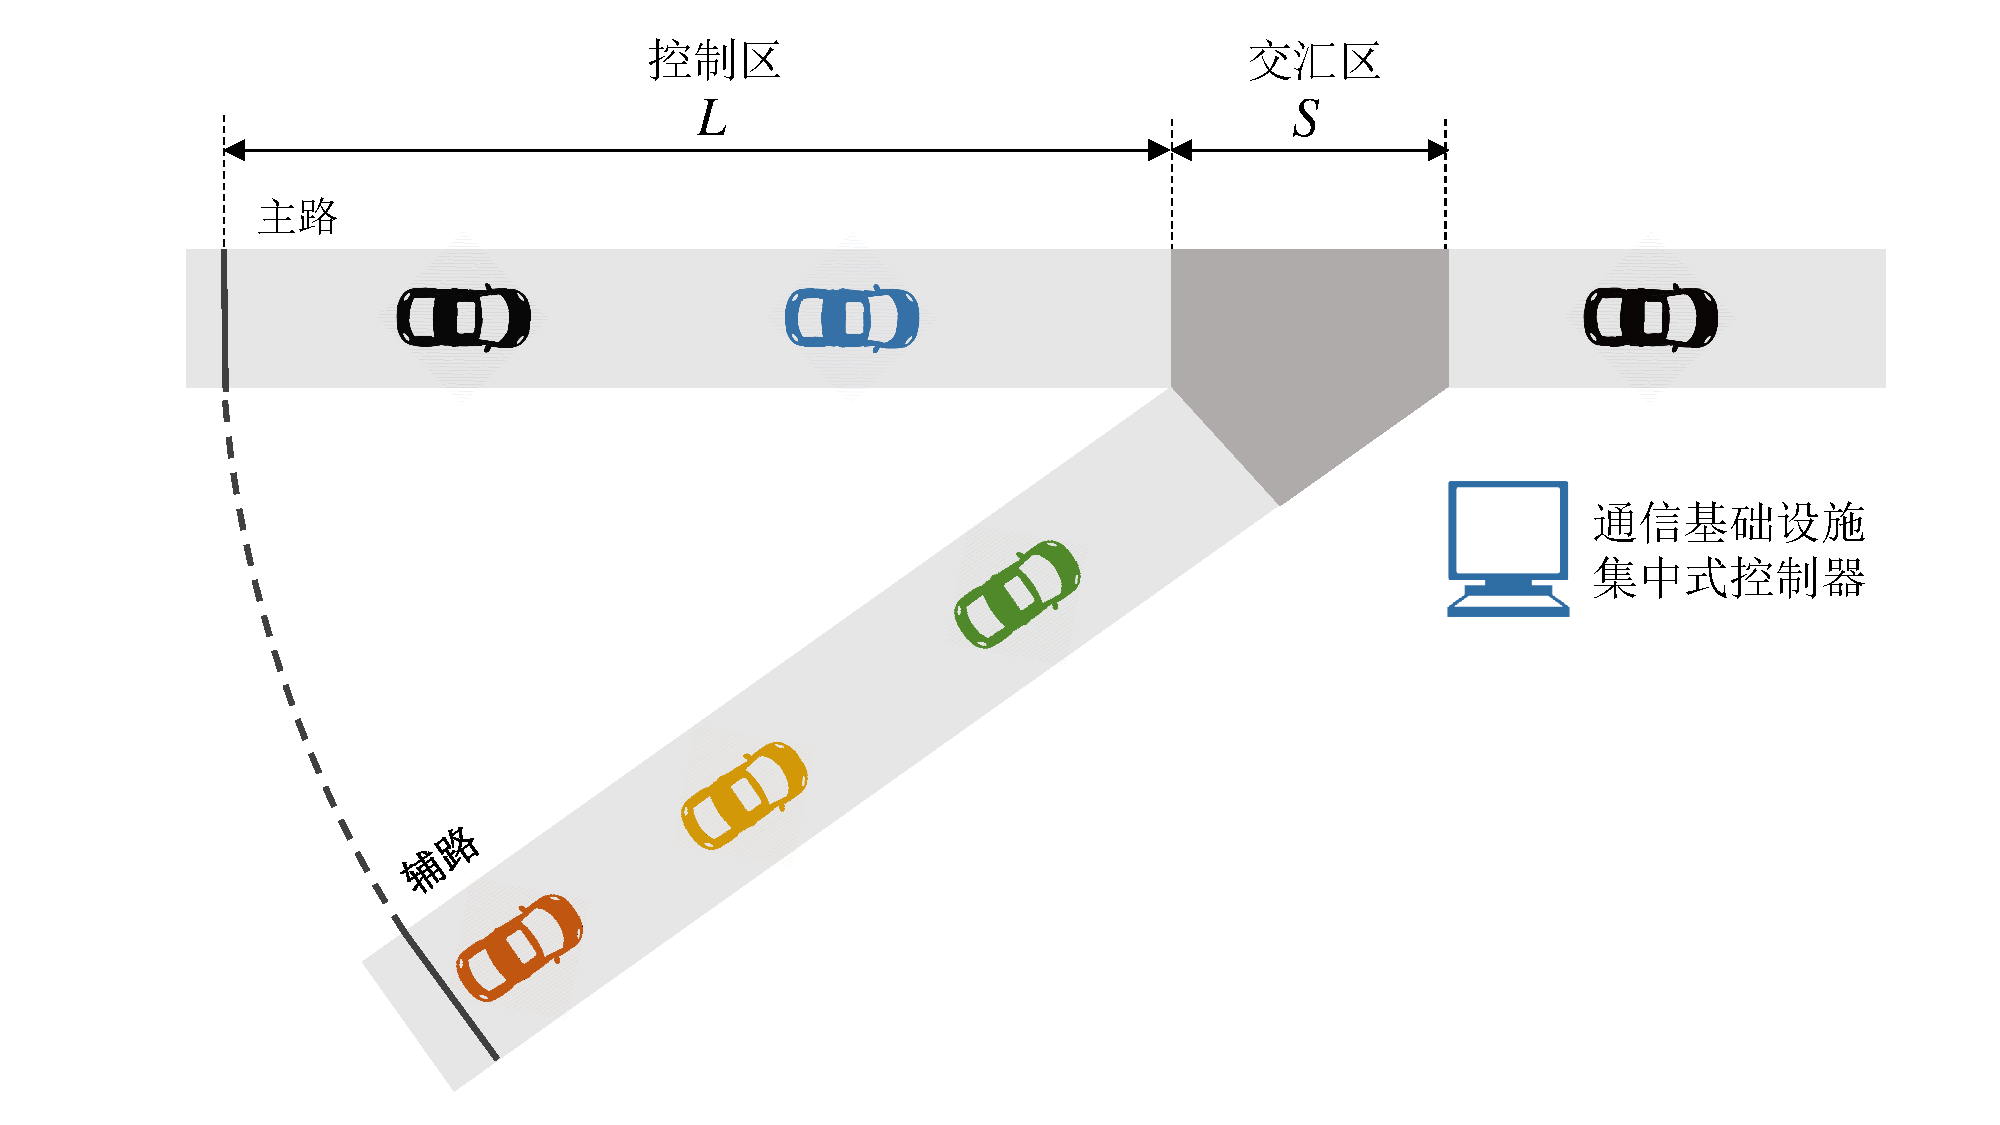
\includegraphics[width=14cm]{../figures/merge.pdf}
\caption{交汇路口示意图}
\label{fig:merge}
\end{figure}

\subsection{车辆状态方程}
假设在时刻 $t$时,位于控制区内的车辆具有某种编号 $\mathcal{N}(t)={1,\dots,N(t)}$,其中 $N(t)$为 $t$时刻控制区内车辆总数。对于每辆车$i\in \mathcal{N}(t)$,系统状态方程为
\begin{equation}
\dot{x}_i=f(t,x_i,u_i),\quad x_i(t_i^0)=x_i^0,
\end{equation}
其中$x_i(t)$,$u_i(t)$分别为第$i$辆车在$t$时刻的状态量和控制量。对于本课题讨论的无人车控制,假定车辆的轨迹已经确定,无需控制方向,只需控制速度。为了保证速度的连续性,选取控制量为加速度,则控制量与状态量的关系为,
\begin{equation}
\begin{gathered}
\dot{p}_i=v_i(t)\\
\dot{v}_i=u_i(t)
\end{gathered}
\end{equation}

其中 $p_i(t)\in \mathcal{P}_i$,$v_i(t)\in \mathcal{V}_i$,$u_i(t)\in \mathcal{U}_i$分别为第 $i$辆车在 $t$时刻的位置,速度和加速度。由于轨迹事先已确定,只需要两个标量 $p_i$与 $v_i$即可确定当前车辆的位置和速度。二者构成了车辆的状态向量 $x_i(t)=[p_i(t), v_i(t)]^\mathrm{T}\in \mathcal{X}_i$,$\mathcal{X}_i=\mathcal{P}\times\mathcal{V}$,并定义进入控制区的初始状态为$x_i^0 = [0, v_i^0]^\mathrm{T}$。

对于实际运行的车辆,其速度和加速度均有限,表达为以下约束,
\begin{equation}
\begin{aligned}
u_{i,\min}\leq u_i(t)\leq u_{i,\max}&, \quad \text{and}\\
0\leq v_{\min}\leq v_i(t)\leq v_{\max}&, \quad \forall t\in[t_i^0, t_i^\mathrm{f}]
\end{aligned}
\label{eq:single_constraint}
\end{equation}
其中 $t_i^\mathrm{f}$为第 $i$辆车离开交汇区的时刻,即控制算法结束的时刻。 $u_{i,\min}$,$u_{i,\max}$分别为第$i$辆车的最小、最大加速度,$v_{\min}$,$v_{\max}$为道路的最低、最高限速。为简单起见,考虑同质车辆,所有CAV均具有相同的最小、最大加速度,即$u_{i,\min}=u_{\min}$,$u_{i,\max}=u_{\max}$。

\subsection{安全性约束与假设}
上一节建立了每辆车的状态方程和单车的约束条件,本节考虑车辆之间的约束关系。

控制算法首先要保证车辆之间不发生追尾。对同一车道上的车辆,定义安全距离$\delta < S$,同车道车辆之间不追尾的约束可以表示为,
\begin{equation}
s_i(t)=p_k(t)-p_i(t)\geq \delta, \ \forall t\in [t_i^0, t_i^\mathrm{f}],
\label{eq:colli_rear}
\end{equation}
其中$k$表示与$i$在同一车道的前一辆车的编号。上式涵盖了控制区、交汇区不发生同车道追尾的约束条件。

车辆仅在交汇区可能与对路车辆发生横向碰撞。给出如下定义:
\begin{definition}
对所有$i\in \mathcal{N}(t)$,定义第 $i$辆车的可能碰撞集 $\Gamma_i$为可能发生横向碰撞的$i$车位置构成的集合,即
\begin{equation}
\Gamma_i\triangleq \{p_i(t)\in[L,L+S],\  \forall t\in [t_i^\mathrm{m},t_i^\mathrm{f}]\}.
\end{equation}
其中$t_i^\mathrm{m}$为第$i$辆车离开控制区,进入交汇区的时刻。
\end{definition}
为了避免横向碰撞,对任意不在同一条路上的两辆车 $\forall i,j\in \mathcal{N}(t)$,给出如下约束:
\begin{equation}
\Gamma_i\cap \Gamma_j=\varnothing, \ \forall t\in [t_i^\mathrm{m},t_i^\mathrm{f}].
\label{eq:colli_lateral}
\end{equation}
上式要求来自相互交汇的两条路上的车辆不能同时出现在交汇区。这个约束必能保证车辆在交汇区不发生横向碰撞,但当交汇区的长度很长时,约束可能过强,没有必要。在下面的章节中将讨论如何放松该约束。

在定义优化目标之前,对控制算法做以下假设。
\begin{assumption}
进入控制区的车$i$满足约束式\ref{eq:single_constraint},\ref{eq:colli_rear}。
\label{ass:restrict}
\end{assumption}
\begin{assumption}
CAV在交汇区保持匀速行驶,且速度相同,即$v_i(t) = v_i(t_i^\mathrm{m}) = v_i(t_i^\mathrm{f}) = v_\mathrm{d}, \ \forall t\in [t_i^\mathrm{m},t_i^\mathrm{f}]$,其中$v_\mathrm{d}$为期望速度。由此可得
\begin{equation}
t_i^\mathrm{f}=t_i^\mathrm{m} + \frac{S}{v_\mathrm{d}}.
\end{equation}
\label{ass:smooth}
\end{assumption}
\begin{assumption}
忽略CAV之间信息传输的延时和错误。
\label{ass:time}
\end{assumption}

在以上假设中,假设\ref{ass:restrict}保证了初始状态的可行性。假设\ref{ass:smooth}忽略了交汇区的速度变化,且假设车辆在进入交汇区之前已经调整到了期望速度$v_\mathrm{d}$。该速度可以根据路段的限速事先给定。这是为了方便讨论交汇区的不碰撞约束,实际情况与此有一定差别。后文将对此展开进一步讨论。假设\ref{ass:time}保证车辆之间信息交互是实时且准确的。但本文的模型在信息的延时和错误处于有限范围内,仍可进行扩展。

\section{群决策算法框架}
% 这里加一段优化目标的综述
\subsection{时间序列的确定}
在假设\ref{ass:smooth}下,考虑到约束式\ref{eq:colli_rear}与式\ref{eq:colli_lateral},可以由$t_{i-1}^\mathrm{m}$确定$t_i^\mathrm{m}$的下界。考虑以下几种情况:
\paragraph{情况一} $i$车与 $i-1$车在同一车道,此时前后车只需保持安全距离,当$i-1$车驶过$\delta$距离后,$i$车便可进入交汇区。由此可得,
\begin{equation}
t_i^\mathrm{m}=t_{i-1}^\mathrm{m} + \frac{\delta}{v_\mathrm{d}}
\end{equation}
\paragraph{情况二}  $i$车与 $i-1$车在不同车道,由式\ref{eq:colli_lateral},当$i-1$车完全驶过交汇区后,$i$车才能进入交汇区。由此可得,
\begin{equation}
t_i^\mathrm{m}=t_{i-1}^\mathrm{m} + \frac{S}{v_\mathrm{d}}
\end{equation}

上述情况二满足了式\ref{eq:colli_lateral}所要求的不同车道不同时出现在交汇区的要求。若交汇区比较长,该要求可以适当放松为,使不同车道间车辆交汇后相距为 $r < S$,$r$为不同车道保证不发生横向碰撞的安全距离。在实际道路条件下,安全距离应随着速度的增加而适当增大。由于交汇区车速仍可视为保持期望速度 $v_\mathrm{d}$,$r$也可以作为常数而预先确定下来。情况二对应的时间关系变为,
\begin{equation}
t_i^\mathrm{m}=t_{i-1}^\mathrm{m} + \frac{r}{v_\mathrm{d}}
\end{equation}

另外,对于不存在前车的第一辆车,其到达交汇区时间 $t_1^\mathrm{m}$可由优化目标解出。这将在下文进一步讨论。

\subsection{优化目标建立}
研究CAV的决策问题,就是在控制量满足一定约束的情况下,对每辆车给出一列控制量输入$u_i(t)$对于车道汇合的场景,一般优化目标包含最小化控制量的输入和最小化平均通行时间。

\subsection{算法可行性论证}
\begin{table}[htb]
  \centering
  \begin{minipage}[t]{0.8\linewidth} % 如果想在表格中使用脚注,minipage是个不错的办法
  \caption[模板文件]{模板文件。如果表格的标题很长,那么在表格索引中就会很不美
    观,所以要像 chapter 那样在前面用中括号写一个简短的标题。这个标题会出现在索
    引中。}
  \label{tab:template-files}
    \begin{tabularx}{\linewidth}{lX}
      \toprule[1.5pt]
      {\heiti 文件名} & {\heiti 描述} \\\midrule[1pt]
      thuthesis.ins & \LaTeX{} 安装文件,\textsc{DocStrip}\footnote{表格中的脚注} \\
      thuthesis.dtx & 所有的一切都在这里面\footnote{再来一个}。\\
      thuthesis.cls & 模板类文件。\\
      thuthesis.cfg & 模板配置文。cls 和 cfg 由前两个文件生成。\\
      thuthesis.bst    & 参考文献 BIB\TeX\ 样式文件。\\
      thuthesis.sty   & 常用的包和命令写在这里,减轻主文件的负担。\\
      \bottomrule[1.5pt]
    \end{tabularx}
  \end{minipage}
\end{table}
\subsection{算法}


%%% 其它部分

\backmatter

%% 本科生要这几个索引,研究生不要。选择性留下。
% 插图索引
\listoffigures
% 表格索引
\listoftables
% 公式索引
\listofequations


%% 参考文献
% 注意:至少需要引用一篇参考文献,否则下面两行可能引起编译错误。
% 如果不需要参考文献,请将下面两行删除或注释掉。
\bibliographystyle{thuthesis-numerical}
\bibliography{ref/refs}


%% 致谢
% 如果使用声明扫描页,将可选参数指定为扫描后的 PDF 文件名,例如:
% \begin{acknowledgement}[scan-statement.pdf]
\begin{acknowledgement}
  衷心感谢导师 张毅 教授对本人的精心指导,与其博士生 封硕 师兄对我的帮助。他们的言传身教将使
  我终生受益。

  特拉华大学(University of Delaware)教授 Andreas Malikopoulos 的多篇文章给了我很大启发,并且详细解释了我对其论文的一些疑问,在此表示感谢。

  感谢我的父母和朋友在我毕设其间对我的帮助和支持。

  感谢 \thuthesis 项目及其维护者们,为我的毕业论文提供了格式和部分技术支持,大大减轻了我论文排版的工作量。
\end{acknowledgement}


%% 附录
\begin{appendix}
\chapter{外文资料原文}
\label{cha:engorg}

\title{The title of the English paper}

\textbf{Abstract:} As one of the most widely used techniques in operations
research, \emph{ mathematical programming} is defined as a means of maximizing a
quantity known as \emph{bjective function}, subject to a set of constraints
represented by equations and inequalities. Some known subtopics of mathematical
programming are linear programming, nonlinear programming, multiobjective
programming, goal programming, dynamic programming, and multilevel
programming$^{[1]}$.

It is impossible to cover in a single chapter every concept of mathematical
programming. This chapter introduces only the basic concepts and techniques of
mathematical programming such that readers gain an understanding of them
throughout the book$^{[2,3]}$.


\section{Single-Objective Programming}
The general form of single-objective programming (SOP) is written
as follows,
\begin{equation}\tag*{(123)} % 如果附录中的公式不想让它出现在公式索引中,那就请
                             % 用 \tag*{xxxx}
\left\{\begin{array}{l}
\max \,\,f(x)\\[0.1 cm]
\mbox{subject to:} \\ [0.1 cm]
\qquad g_j(x)\le 0,\quad j=1,2,\cdots,p
\end{array}\right.
\end{equation}
which maximizes a real-valued function $f$ of
$x=(x_1,x_2,\cdots,x_n)$ subject to a set of constraints.

\newtheorem{mpdef}{Definition}[chapter]
\begin{mpdef}
In SOP, we call $x$ a decision vector, and
$x_1,x_2,\cdots,x_n$ decision variables. The function
$f$ is called the objective function. The set
\begin{equation}\tag*{(456)} % 这里同理,其它不再一一指定。
S=\left\{x\in\Re^n\bigm|g_j(x)\le 0,\,j=1,2,\cdots,p\right\}
\end{equation}
is called the feasible set. An element $x$ in $S$ is called a
feasible solution.
\end{mpdef}

\newtheorem{mpdefop}[mpdef]{Definition}
\begin{mpdefop}
A feasible solution $x^*$ is called the optimal
solution of SOP if and only if
\begin{equation}
f(x^*)\ge f(x)
\end{equation}
for any feasible solution $x$.
\end{mpdefop}

One of the outstanding contributions to mathematical programming was known as
the Kuhn-Tucker conditions\ref{eq:ktc}. In order to introduce them, let us give
some definitions. An inequality constraint $g_j(x)\le 0$ is said to be active at
a point $x^*$ if $g_j(x^*)=0$. A point $x^*$ satisfying $g_j(x^*)\le 0$ is said
to be regular if the gradient vectors $\nabla g_j(x)$ of all active constraints
are linearly independent.

Let $x^*$ be a regular point of the constraints of SOP and assume that all the
functions $f(x)$ and $g_j(x),j=1,2,\cdots,p$ are differentiable. If $x^*$ is a
local optimal solution, then there exist Lagrange multipliers
$\lambda_j,j=1,2,\cdots,p$ such that the following Kuhn-Tucker conditions hold,
\begin{equation}
\label{eq:ktc}
\left\{\begin{array}{l}
    \nabla f(x^*)-\sum\limits_{j=1}^p\lambda_j\nabla g_j(x^*)=0\\[0.3cm]
    \lambda_jg_j(x^*)=0,\quad j=1,2,\cdots,p\\[0.2cm]
    \lambda_j\ge 0,\quad j=1,2,\cdots,p.
\end{array}\right.
\end{equation}
If all the functions $f(x)$ and $g_j(x),j=1,2,\cdots,p$ are convex and
differentiable, and the point $x^*$ satisfies the Kuhn-Tucker conditions
(\ref{eq:ktc}), then it has been proved that the point $x^*$ is a global optimal
solution of SOP.

\subsection{Linear Programming}
\label{sec:lp}

If the functions $f(x),g_j(x),j=1,2,\cdots,p$ are all linear, then SOP is called
a {\em linear programming}.

The feasible set of linear is always convex. A point $x$ is called an extreme
point of convex set $S$ if $x\in S$ and $x$ cannot be expressed as a convex
combination of two points in $S$. It has been shown that the optimal solution to
linear programming corresponds to an extreme point of its feasible set provided
that the feasible set $S$ is bounded. This fact is the basis of the {\em simplex
  algorithm} which was developed by Dantzig as a very efficient method for
solving linear programming.
\begin{table}[ht]
\centering
  \centering
  \caption*{Table~1\hskip1em This is an example for manually numbered table, which
    would not appear in the list of tables}
  \label{tab:badtabular2}
  \begin{tabular}[c]{|m{1.5cm}|c|c|c|c|c|c|}\hline
    \multicolumn{2}{|c|}{Network Topology} & \# of nodes &
    \multicolumn{3}{c|}{\# of clients} & Server \\\hline
    GT-ITM & Waxman Transit-Stub & 600 &
    \multirow{2}{2em}{2\%}&
    \multirow{2}{2em}{10\%}&
    \multirow{2}{2em}{50\%}&
    \multirow{2}{1.2in}{Max. Connectivity}\\\cline{1-3}
    \multicolumn{2}{|c|}{Inet-2.1} & 6000 & & & &\\\hline
    \multirow{2}{1.5cm}{Xue} & Rui  & Ni &\multicolumn{4}{c|}{\multirow{2}*{\thuthesis}}\\\cline{2-3}
    & \multicolumn{2}{c|}{ABCDEF} &\multicolumn{4}{c|}{} \\\hline
\end{tabular}
\end{table}

Roughly speaking, the simplex algorithm examines only the extreme points of the
feasible set, rather than all feasible points. At first, the simplex algorithm
selects an extreme point as the initial point. The successive extreme point is
selected so as to improve the objective function value. The procedure is
repeated until no improvement in objective function value can be made. The last
extreme point is the optimal solution.

\subsection{Nonlinear Programming}

If at least one of the functions $f(x),g_j(x),j=1,2,\cdots,p$ is nonlinear, then
SOP is called a {\em nonlinear programming}.

A large number of classical optimization methods have been developed to treat
special-structural nonlinear programming based on the mathematical theory
concerned with analyzing the structure of problems.
\begin{figure}[h]
  \centering
  \includegraphics{thu-lib-logo}
  \caption*{Figure~1\quad This is an example for manually numbered figure,
    which would not appear in the list of figures}
  \label{tab:badfigure2}
\end{figure}

Now we consider a nonlinear programming which is confronted solely with
maximizing a real-valued function with domain $\Re^n$.  Whether derivatives are
available or not, the usual strategy is first to select a point in $\Re^n$ which
is thought to be the most likely place where the maximum exists. If there is no
information available on which to base such a selection, a point is chosen at
random. From this first point an attempt is made to construct a sequence of
points, each of which yields an improved objective function value over its
predecessor. The next point to be added to the sequence is chosen by analyzing
the behavior of the function at the previous points. This construction continues
until some termination criterion is met. Methods based upon this strategy are
called {\em ascent methods}, which can be classified as {\em direct methods},
{\em gradient methods}, and {\em Hessian methods} according to the information
about the behavior of objective function $f$. Direct methods require only that
the function can be evaluated at each point. Gradient methods require the
evaluation of first derivatives of $f$. Hessian methods require the evaluation
of second derivatives. In fact, there is no superior method for all
problems. The efficiency of a method is very much dependent upon the objective
function.

\subsection{Integer Programming}

{\em Integer programming} is a special mathematical programming in which all of
the variables are assumed to be only integer values. When there are not only
integer variables but also conventional continuous variables, we call it {\em
  mixed integer programming}. If all the variables are assumed either 0 or 1,
then the problem is termed a {\em zero-one programming}. Although integer
programming can be solved by an {\em exhaustive enumeration} theoretically, it
is impractical to solve realistically sized integer programming problems. The
most successful algorithm so far found to solve integer programming is called
the {\em branch-and-bound enumeration} developed by Balas (1965) and Dakin
(1965). The other technique to integer programming is the {\em cutting plane
  method} developed by Gomory (1959).

\hfill\textit{Uncertain Programming\/}\quad(\textsl{BaoDing Liu, 2006.2})

\section*{References}
\noindent{\itshape NOTE: These references are only for demonstration. They are
  not real citations in the original text.}

\begin{translationbib}
\item Donald E. Knuth. The \TeX book. Addison-Wesley, 1984. ISBN: 0-201-13448-9
\item Paul W. Abrahams, Karl Berry and Kathryn A. Hargreaves. \TeX\ for the
  Impatient. Addison-Wesley, 1990. ISBN: 0-201-51375-7
\item David Salomon. The advanced \TeX book.  New York : Springer, 1995. ISBN:0-387-94556-3
\end{translationbib}

\chapter{外文资料的调研阅读报告或书面翻译}

\title{城市道路自动驾驶车辆运动计划和控制研究综述}

{\heiti 摘要:} 自动驾驶车是一种成熟的技术,通过提高汽车运输的安全性,可及性,效率和便利性,有可能重塑人们的出行方式。 自驾车必须在确保安全的前提下执行任务,包括通过与其他车辆和行人共享的动态环境进行动作规划,以及通过反馈控制可靠地执行动作。 本文的目的是调查目前的规划和控制算法的现状,特别是在城市环境中。本文对部分所提出的技术进行了综述,并讨论了其有效性。 所调查的方法在所使用的车辆移动性模型,环境结构假设和计算要求方面不同。 本次调查中的并列比较有助于深入了解经过调查的方法的优势和局限性,并辅助系统级设计选择。

\section{介绍}

过去三十年来,学术界和工业界都在不断开展无人驾驶技术的研究工作。传感和计算技术的最新进展,无人驾驶技术对汽车运输的潜在转变及其社会效益,推动了这项技术的发展:2014年有交通相关死亡人员32,675人,其中230万人受伤,610万起交通事故被报道[1]。其中,估计有94\%的事故是由驾驶员操作失误造成,31\%涉及饮酒的驾驶员,10\%涉及分心的驾驶员[2]。自动驾驶车有可能大大减少因驾驶员犯错和疏忽而造成的事故。它们还将为由于身体或视觉残疾而无法驾驶的人提供私人交通工具。最后,全美工作人口86\%的人每天平均花25分钟(单程)的时间乘汽车上下班,自动驾驶车将有助于更有效地利用通勤时间,或简单地减少驾驶压力带来的不良影响[4]。

考虑到这种新技术的潜在影响,自驾车已经有悠久的历史。这个想法早在20世纪20年代就已经存在,但直到20世纪80年代,无人驾驶的汽车才真正成为可能。 20世纪80年代由恩斯特·迪克曼(Ernst Dickmanns)(例如[5])领导的开创性工作为无人车的开发铺平了道路。那时候,PROMETHEUS项目的大量研究力量投入了无人车的研发。 1994年,由VaMP开发的无人驾驶汽车驾驶1600公里,其中95\%是自主驾驶[6]。在同一时期,CMU NAVLAB正在该领域取得进展,并在1995年展示了进一步的进展,在5000公里穿越美国的车程中,98\%是自主驾驶[7]。

无人驾驶汽车技术的下一个重大里程碑是2004年第一次DARPA大挑战赛。比赛目标是让无人驾驶汽车尽快通过150英里的越野赛道。与以前的展示相比,这是一个重大的挑战,因为在比赛中不会有人为的干预。虽然以前的工作能实现几乎自主的驾驶,但在关键时刻消除人为干预被证明是一个重大的挑战。15辆车中没有一辆完成比赛。 2005年举办了类似的活动;这一次,23支队伍中有5个到达了终点线[8]。后来,2007年,DARPA城市挑战赛举行,车辆被要求在模拟城市环境中自主驾驶。六个小组完成了这一比赛,表明完全自主的城市驾驶是可能的[9]。

自从DARPA挑战以来,全世界已经进行了许多比赛和较大的无人车系统测试。值得注意的例子包括2009年至2013年的智能车辆未来挑战赛[10],2010年的现代汽车无人车挑战赛[11],2010年的VisLab洲际无人车挑战赛[12],2013年的城市无人驾驶汽车公路测试[13],以及Bertha-Benz路线的自主驾驶测试[14]。同时,在学术环境的改善和行业发展的驱动下,无人车研究工作进展顺利。 Google自驾车[15]和特斯拉的自动驾驶仪系统[16]是获得广泛关注的商业活动的两个例子。

汽车自动化的程度可以从完全由人操作到完全自主操作。 SAE J3016标准[17]引入了从0到5的等级分级车辆自动化程度。在这个标准中,0级代表车辆所有驾驶任务都是人类驾驶员完成。1级包括基本驾驶辅助,如自适应巡航控制,防抱死制动系统和电子稳定控制[18]。2级包括高级辅助系统,如危害最小化纵向/横向控制[19]和紧急制动[20],[21],这些系统通常基于预先设定形式的控制理论来计算“最坏情况” (安全)状态[22] - [24],确保车辆无碰撞。在3级系统中,系统对行车环境进行监控,并且可以在某些条件下完全自主地运行,但如果驾驶任务离开自主系统的操作范围,则仍然需要操作人员进行控制。具有4级自动化的车辆能够在某些条件下完全自主驾驶,并且如果操作者没有根据要求进行干预,仍可以安全地控制车辆。 5级系统在所有驾驶模式下都是完全自主的。

车载计算和无线通信技术的可用性允许汽车与其他车辆和道路基础设施交换信息,引发了与之密切相关的智能网联车技术的研究[25]。这方面研究旨在通过个别车辆之间的信息共享和协调来提高道路运输的安全性和性能。例如,网联车技术有可能改善交叉点处的吞吐量[26]或阻止交通冲击波的形成[27]。

为了限制本次调查的范围,我们专注于自主驾驶汽车的决策,运动规划和控制方面,特别是对于3级及以上的自动化系统。出于同样的原因,自动驾驶车的感知技术被忽略,读者可以参考关于这一主题的一些综述和近期的重要进展[28] - [31]。

当代自主驾驶系统的决策通常分层次地组织成路线规划,行为决策,局部运动规划和反馈控制。然而,文献中有许多不同的划分,因此对决策级别的划分相当模糊。本文对于解决这些自主驾驶核心问题所提出的方法展开了调查,特别强调局部运动规划和控制的方法。

本文的其余部分结构如下:第二部分对决策过程层次进行了概述,展示了部分设计方法。第三节回顾了用于在城市环境中估计汽车的移动性的模型,以便进行运动规划和反馈控制的研究。第四节调查有关运动规划的丰富文献,并讨论其对自驾车的适用性。同样,第五节讨论了无人驾驶汽车的路径和轨迹稳定问题以及具体的反馈控制方法。最后,第六部分总结了并评述了研究现状和未来研究方向。


\section{无人车决策层次概述}

在本节中,我们将描述典型自驾车的决策层次,并对每个部分的功能进行描述。无人驾驶汽车本质上是自动决策系统,可处理来自车载传感器(如雷达,LIDAR,摄像机,GPS / INS单元和测距仪)的观测数据流。这些观察结果以及关于道路网络的现有知识,道路规则,车辆动力学和传感器模型被用于自动选择控制车辆运动的控制变量的值。智能车辆研究旨在尽可能多地自动化驾驶任务。该问题通常采用的方法是将感知和决策任务分解和组织成一个层次结构。感知系统使用先前的信息和收集的观测数据来提供车辆状态及对周围环境的估计,然后由决策系统使用估计来控制车辆,从而完成驾驶目标。

典型自驾车的决策系统被分层分解为四个组成部分(参见图\ref{fig:decision}):在最高层,路线是通过道路网计划的。这之后是一个行为层,决定了一个局部的驾驶任务,逐渐将汽车导向目的地,并兼顾交通规则。运动规划模块然后在通行环境中规划一条连续路径以完成局部导航任务。最后由控制系统在运动的执行中反馈性地纠正错误。在本节的其余部分,我们将更详细地讨论每个部分的功能。

\begin{figure}
\centering
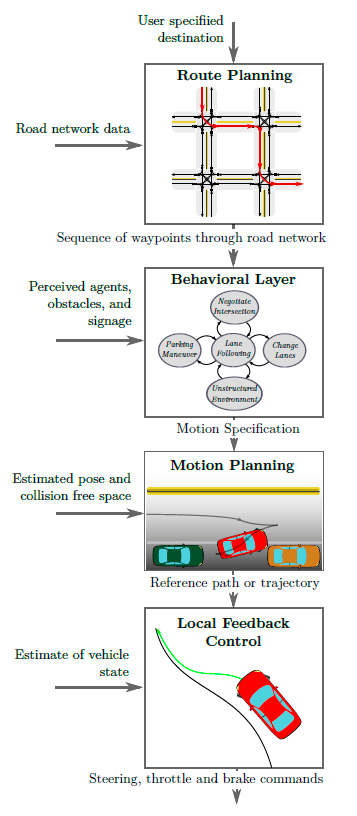
\includegraphics[width=8cm]{decision.png}
\caption{无人车决策层级图}
\caption*{目的地作为路径规划层的输入,生成路网上的路径。行为决策层根据该路径和周围环境,生成一列指向目的地的具体行动。运动规划层进而规划出完成该行动的可行路径。反馈控制调整执行变量以纠正执行参考路径中的错误。}
\label{fig:decision}
\end{figure}

\subsection{路径规划}
在最高级别,车辆的决策系统必须选择通过道路网从当前位置到所要求的目的地的路线。通过将道路网络表示为具有与穿越该路段的成本相对应的赋权有向图,可以将路径规划问题转化为在道路网络图上找到最小成本路径的问题。然而,代表道路网络的图形可以包含数百万条边,使得经典的最短路径算法(如Dijkstra [32]或A * [33])不切实际。运输网络中高效路线规划的问题引起了运输科学界的极大兴趣,研究者发明了一系列算法,经过一次性预处理步骤,可以在几毫秒内在大陆规模的网络上返回最佳路径[34],[35]。对于可用于有效规划驾驶员驾驶和自动驾驶车路线的实际算法的综合调查和比较,参见[36]。

\subsection{行为决策}
在找到路线之后,无人车必须能够根据交通规则,导航所选择的路线,并与其他交通参与者进行交互。给定指示所选路线的路段的序列,行为决策层负责根据其他交通参与者的感知行为,路况和基础设施的信号在任意时间点选择合适的驾驶行为。例如,当车辆在交叉口前到达停车线时,行为层将命令车辆停下来,观察交叉路口处的其他车辆,自行车和行人的行为,并当轮到本车运行时发出运行指令。驾驶手册规定了具体驾驶环境的定性动作。由于驾驶环境和每个环境中可用的行为都可以被建模为有限集,自动化这种决策的自然方法是将每个行为建模成有限状态机中的状态,其中转移由感知到的驾驶环境控制,如本车相对于计划路线和附近车辆的位置。事实上,DARPA城市挑战中大多数团队都采用了有限状态机与特定于驾驶场景的不同启发式搜索[9]作为行为控制机制。

然而,现实世界的驾驶,特别是在城市中,其他交通参与者的意图不确定。研究者们还研究了其他车辆,自行车和行人未来轨迹的意图预测和估计问题。所提出的解决方案是基于机器学习的技术,例如高斯混合模型[37],高斯过程回归[38](这种方法被用于Google自主驾驶系统中意图预测的学习[39]),以及基于模型的直接从传感器测量数据估计意图的方法[40],[41]。

其他交通参与者的行为中的这种不确定性在行为决策层中通常建模为概率模型(例如马尔可夫决策过程(MDP))。例如,[42]在MDP框架中制定行为决策。一些工作[43] - [46]将未观察到的驾驶场景和行人意图显式建模为部分可观察的马尔可夫决策过程(POMDP),并提出具体的求近似解的策略。

\subsection{运动规划}
当行为层决定在当前环境中执行的驾驶行为,例如跟驰,换道或右转时,所选择的行为必须被转换为路径或轨迹,才可以由低级反馈控制器跟踪。所得到的路径或轨迹必须对于车辆而言是动态可行的,对于乘客来说舒适,并且避免与车载传感器检测到的障碍物的碰撞。找到这样的路径或轨迹是运动规划系统的任务。

无人车的运动规划任务与机器人控制相关文献中讨论的求解标准运动规划的问题密切相关。在大多数情况下,运动规划问题的精确解决方案在计算上是不可行的。因此,在实践中通常使用数值近似方法。最常用的数值方法有变分法、图搜索发和增量树法等。其中变分法将轨迹求解问题转化为函数空间中的非线性优化问题;图搜索方法将构成车辆状态空间的道路拓扑图离散化并搜索最短路径;增量树法从车辆的初始状态逐渐构建可达状态树,然后选择这样一棵树的最佳分支。自动驾驶相关的运动规划方法在第四节中有更详细的讨论。

\subsection{车辆控制}
为了执行运动规划系统确定的参考路径或轨迹,无人车使用反馈控制器来选择适当的执行器输入以执行计划的运动和纠正跟踪误差。 执行计划运动期间产生的跟踪误差部分原因在于车辆模型的不准确。 因此,闭环系统的鲁棒性和稳定性非常重要。

研究者们已经设计了许多有效的反馈控制器,来执行由运动规划系统提供的参考路径或轨迹。 相关技术在第五节中有详细的讨论。

\section{无人车运动模型}
在本节中,我们将调查最常用的车辆运动模型。这些模型被广泛用于控制和运动规划算法中,来近似车辆的行为,响应相关操作条件下的控制动作。高保真模型可以准确反映车辆对控制量输入的响应,但是附加的细节可能使计划和控制问题复杂化。这提供了所选模型的准确性与决策问题的难度之间的权衡。本节概述了一般建模概念和运动规划和控制模型。

建模从车辆配置的概念开始,代表其在世界上的姿势或位置。例如,配置可以表示为汽车上的点与汽车的航向的平面坐标。这是汽车配置空间的坐标系。该坐标系描述平面刚体运动(由特殊欧几里德组在两维中表示,SE(2)),并且是常用的配置空间[47] - [49]。车辆运动的规划和调整必须在遵循所选模型引入的限制的前提下,完成驾驶任务。

\subsection{单轨道运动学模型}
在实际使用的最基本模型中,汽车由两个通过刚性连杆连接的轮子组成,并被限制在一个平面上移动[48] - [52]。 假设车轮在与地面的接触点处不会滑动,而可以绕其旋转轴线自由旋转。 前轮具有附加的自由度,允许其绕垂直于运动平面的轴线旋转,以对转向进行建模。 该模型的这两个特征反映了大多数乘客在不同时前进的情况下不能进行横向位移的经验。 更正式地说,这种机动性的限制被称为非完整约束[47],[53]。 非完整约束被表示为对汽车运动的差分约束。 该表达式取决于坐标系的选择。 该模型的各种变种通常被称为类车机器人,自行车模型,运动模型或单轨道模型。

以下是用于配置的几个常用坐标系中差分约束的推导。 参考图\ref{fig:kinematics},矢量$p_r$和$p_f$表示后轮和前轮在具有基矢量$(\hat{e}_x, \hat{e}_y, \hat{e}_z)$的静止或惯性坐标系中的位置。朝向角$\theta$是描述车辆所面向的方向的角度,定义为向量$\hat{e}_x$和$p_f-p_r$之间的角度。
\begin{figure}
\centering
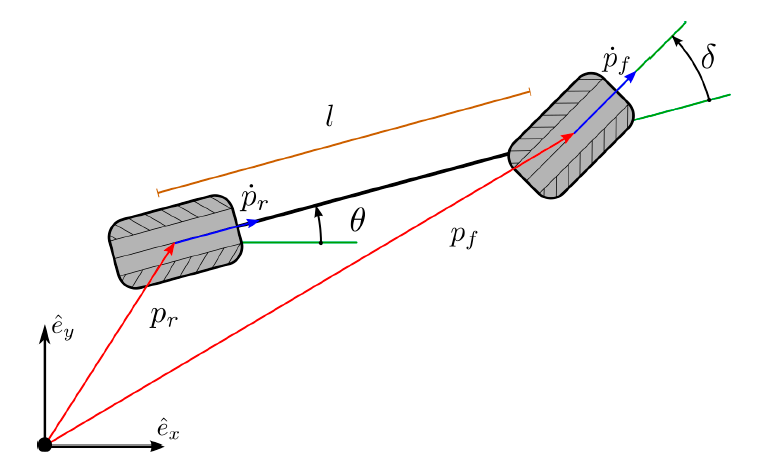
\includegraphics[width=13cm]{kinematics.png}
\caption{单轨道运动学模型图}
\caption*{$p_r$与$p_f$分别为后轮、前轮与地面的触点,$\theta$是车辆朝向角。$p_r$与$p_f$对时间的导数的方向受到非完整性约束的限制,如图中蓝色箭头所示。$\delta$是前轮导向角。}
\label{fig:kinematics}
\end{figure}

下面将对于包含朝向角$\theta$,点$p_r$的运动,点$p_f$的运动的坐标系导出差分约束。

为了满足接触点不滑动的约束,点$p_r$,$p_f$的运动必须与轮子的朝向共线,对后轮,该约束表示为
\begin{equation}
(\dot{p}_r\cdot \hat{e}_y)\cos(\theta)-(\dot{p}_r\cdot \hat{e}_x)\sin(\theta)=0,
\end{equation}
对前轮,有
\begin{equation}
(\dot{p}_f\cdot \hat{e}_y)\cos(\theta+\delta)-(\dot{p}_f\cdot \hat{e}_x)\sin(\theta+\delta)=0.
\end{equation}
该表达式通常被重写为关于基向量的分量形式。后轮运动在$\hat{e}_x$方向的分量为$x_r := p_r\cdot\hat{e}_x$,在$\hat{e}_y$方向为$y_r:=p_r\cdot \hat{e}_y$。前进速度为$v_r:=\dot{p}_r\cdot(p_f-p_r)/\|(p_f-p_r)\|$,即$\dot{p}_r$的模长乘上表示方向的符号。关于标量$x_r$,$y_r$和$\theta$,差分约束表示为
\begin{align}
\begin{split}
\dot{x}_r&= v_r\cos(\theta),\\
\dot{y}_r&= v_r\sin(\theta),\\
\dot{\theta}&=\frac{v_r}{l}\tan(\delta).
\end{split}
\end{align}
同样,对于点$p_f$的运动也具有差分约束
\begin{align}
\begin{split}
\dot{x}_f&= v_f\cos(\theta),\\
\dot{y}_f&= v_f\sin(\theta),\\
\dot{\theta}&=\frac{v_f}{l}\tan(\delta).
\end{split}
\label{eq:vf}
\end{align}
其中,前轮速度$v_f$与后轮速度有关系
\begin{equation}
\frac{v_r}{v_f}=\cos(\delta).
\end{equation}

对该车辆模型的规划和控制需要决定前轮导向角$\delta\in [\delta_{\min}, \delta_{\max}]$和前进速度$v_r\in [v_{\min}, v_{\max}]$。

一个常用的简化,如在[56]中用到的,是选择航向率$\omega$,而不是导向角$\delta$。二者存在关系
\begin{equation}
\delta=\arctan(\frac{l\omega}{v_r})
\end{equation}
这将朝向的运动简化为
\begin{equation}
\dot{\theta}=\omega, \quad \omega\in [\frac{v_r}{l}\tan(\delta_{\min}, \frac{v_r}{l}\tan(\delta_{\max})]
\end{equation}
这种模型有时被称为单轮车模型,因为它可以通过考虑单个车轮的运动而得出。

单轨道运动模型的一个重要变种是固定$v_r$的情况。 这有时被称为杜宾斯车,以莱斯特·杜宾斯(Lester Dubins)命名,他在规定切线的情形下得出了两点之间的最短时间运动[57]。另一个重要变种是Reed-Shepp车,当$v_r$取单值的正向和反向速度时,可以求出最小长度的路径[58]。 这两个模型已被证明对运动规划具有重要意义,并将在第四节进一步讨论。

运动学模型适用于低速情形,例如停车机动和城市驾驶。在该情形下车的惯性较小,不足以打破车轮不打滑的假设。该模型的主要缺点是它允许转向角度瞬间变化。如果运动计划模块要求产生这种瞬时变化,这将是有问题的。

转向角的连续性可以通过改进(\ref{eq:vf})来实现,其中转向角是转角速率的积分,如[49]所示。 方程式(\ref{eq:vf})变为
\begin{align}
\begin{split}
\dot{x}_f&= v_f\cos(\theta),\\
\dot{y}_f&= v_f\sin(\theta),\\
\dot{\theta}&=\frac{v_f}{l}\tan(\delta),\\
\dot{\delta}&=v_{\delta}.
\end{split}
\end{align}
除了对导向角的连续性限制,转角变化率也可以引入约束$v_{\delta}\in [\dot{\delta}_{\min},\dot{\delta}_{\max}]$。同样的问题也会出现在速度控制上。可以通过引入加速度保证速度控制的连续性。这种方法的缺点在于增加了模型的维数,将运动计划与控制问题变得更为复杂。

坐标系的选择不限于使用一个车轮位置作为位置坐标。 对于使用经典力学原理得出的模型,可以使用质心作为位置坐标,如[59],[60]或使用振荡中心,如[61],[62]。

\chapter{其它附录}
前面两个附录主要是给本科生做例子。其它附录的内容可以放到这里,当然如果你愿意,可
以把这部分也放到独立的文件中,然后将其 \cs{input} 到主文件中。

\end{appendix}

%% 个人简历
\include{data/resume}

%% 本科生进行格式审查是需要下面这个表格,答辩可能不需要。选择性留下。
% 综合论文训练记录表
\includepdf[pages=-]{scan-record.pdf}
\end{document}
